\chapter{Experimental methods}
% -------------------------
%% QUOTE
\vspace*{\fill}
\epigraph{As thou sowest, so shalt thou reap.}%
{\textit{De Oratore, II. 65. in Hoyt's New Cyclopedia Of Practical Quotations}\\ \textsc{Cisero}}
\clearpage{\thispagestyle{empty}\cleardoublepage}
%%
%% Body of the chapter
%%%%%%%%%%%%%%%%%%%%%%
This chapter provides an overview of experimental systems and procedures implemented in data acquisition throughout the project. Detailed description of used methods are given, where applicable, and their respective results are presented in Chapter \ref{chap:results}.

\section{PEC nanogels} \index{polyelectrolyte complexes}
\subsection{Objective}
As explained earlier in Chapter \ref{chap:background}, a polyelectrolyte complex (PEC) is a nanoparticle that can be formed by mixing a polyanion and a polycation. Both constituents can be polymers with low molecular weights. Once the PEC is formed, an active ingredient (e.g. \ce{Cr^3+}) can be encapsulated into it, which will be later used to cross link polymers such as HPAM.

A research group at Texas A\&M\footnote{The research was originally conducted at University of Kansas. However, since Professor Jenn-Tai Liang, one of the contributors to this project and HyGreGel, later moved to Texas A\&M University, we will call it a Texas A\&M recipe here.} has developed a technology to delay gelation of HPAM based on PEC and \ce{Cr^3+}. Only a few works have been published on their results \citep[e.g.][]{Cordova2008,Johnson2010}. Figure \ref{cht:jennTai} shows an example of a system with delayed gelation based on Texas A\&M technology. As shown in the figure, the viscosity of the solution only increased marginally for the first 50 days after preparation. Then after 50 days, a sudden viscosity increase of several orders of magnitude was observed over a 10 day period.

As active amine POSS nanoparticles are on type of polycations, it was proposed by Texas A\&M that amine POSS could possibly be used as polycation for PEC in the HyGreGel project. In this way there will be no need to add a third constituent as the nanoparticle also serves as the cross linker. This could possibly result in a more robust system for practical use as the system only includes two components. Initial measurements at Texas A\&M indicated that this could be a viable path to follow.

Therefore, several types of PEC nanogels were prepared and measured in order to test the idea.

\begin{figure}
    \centering
    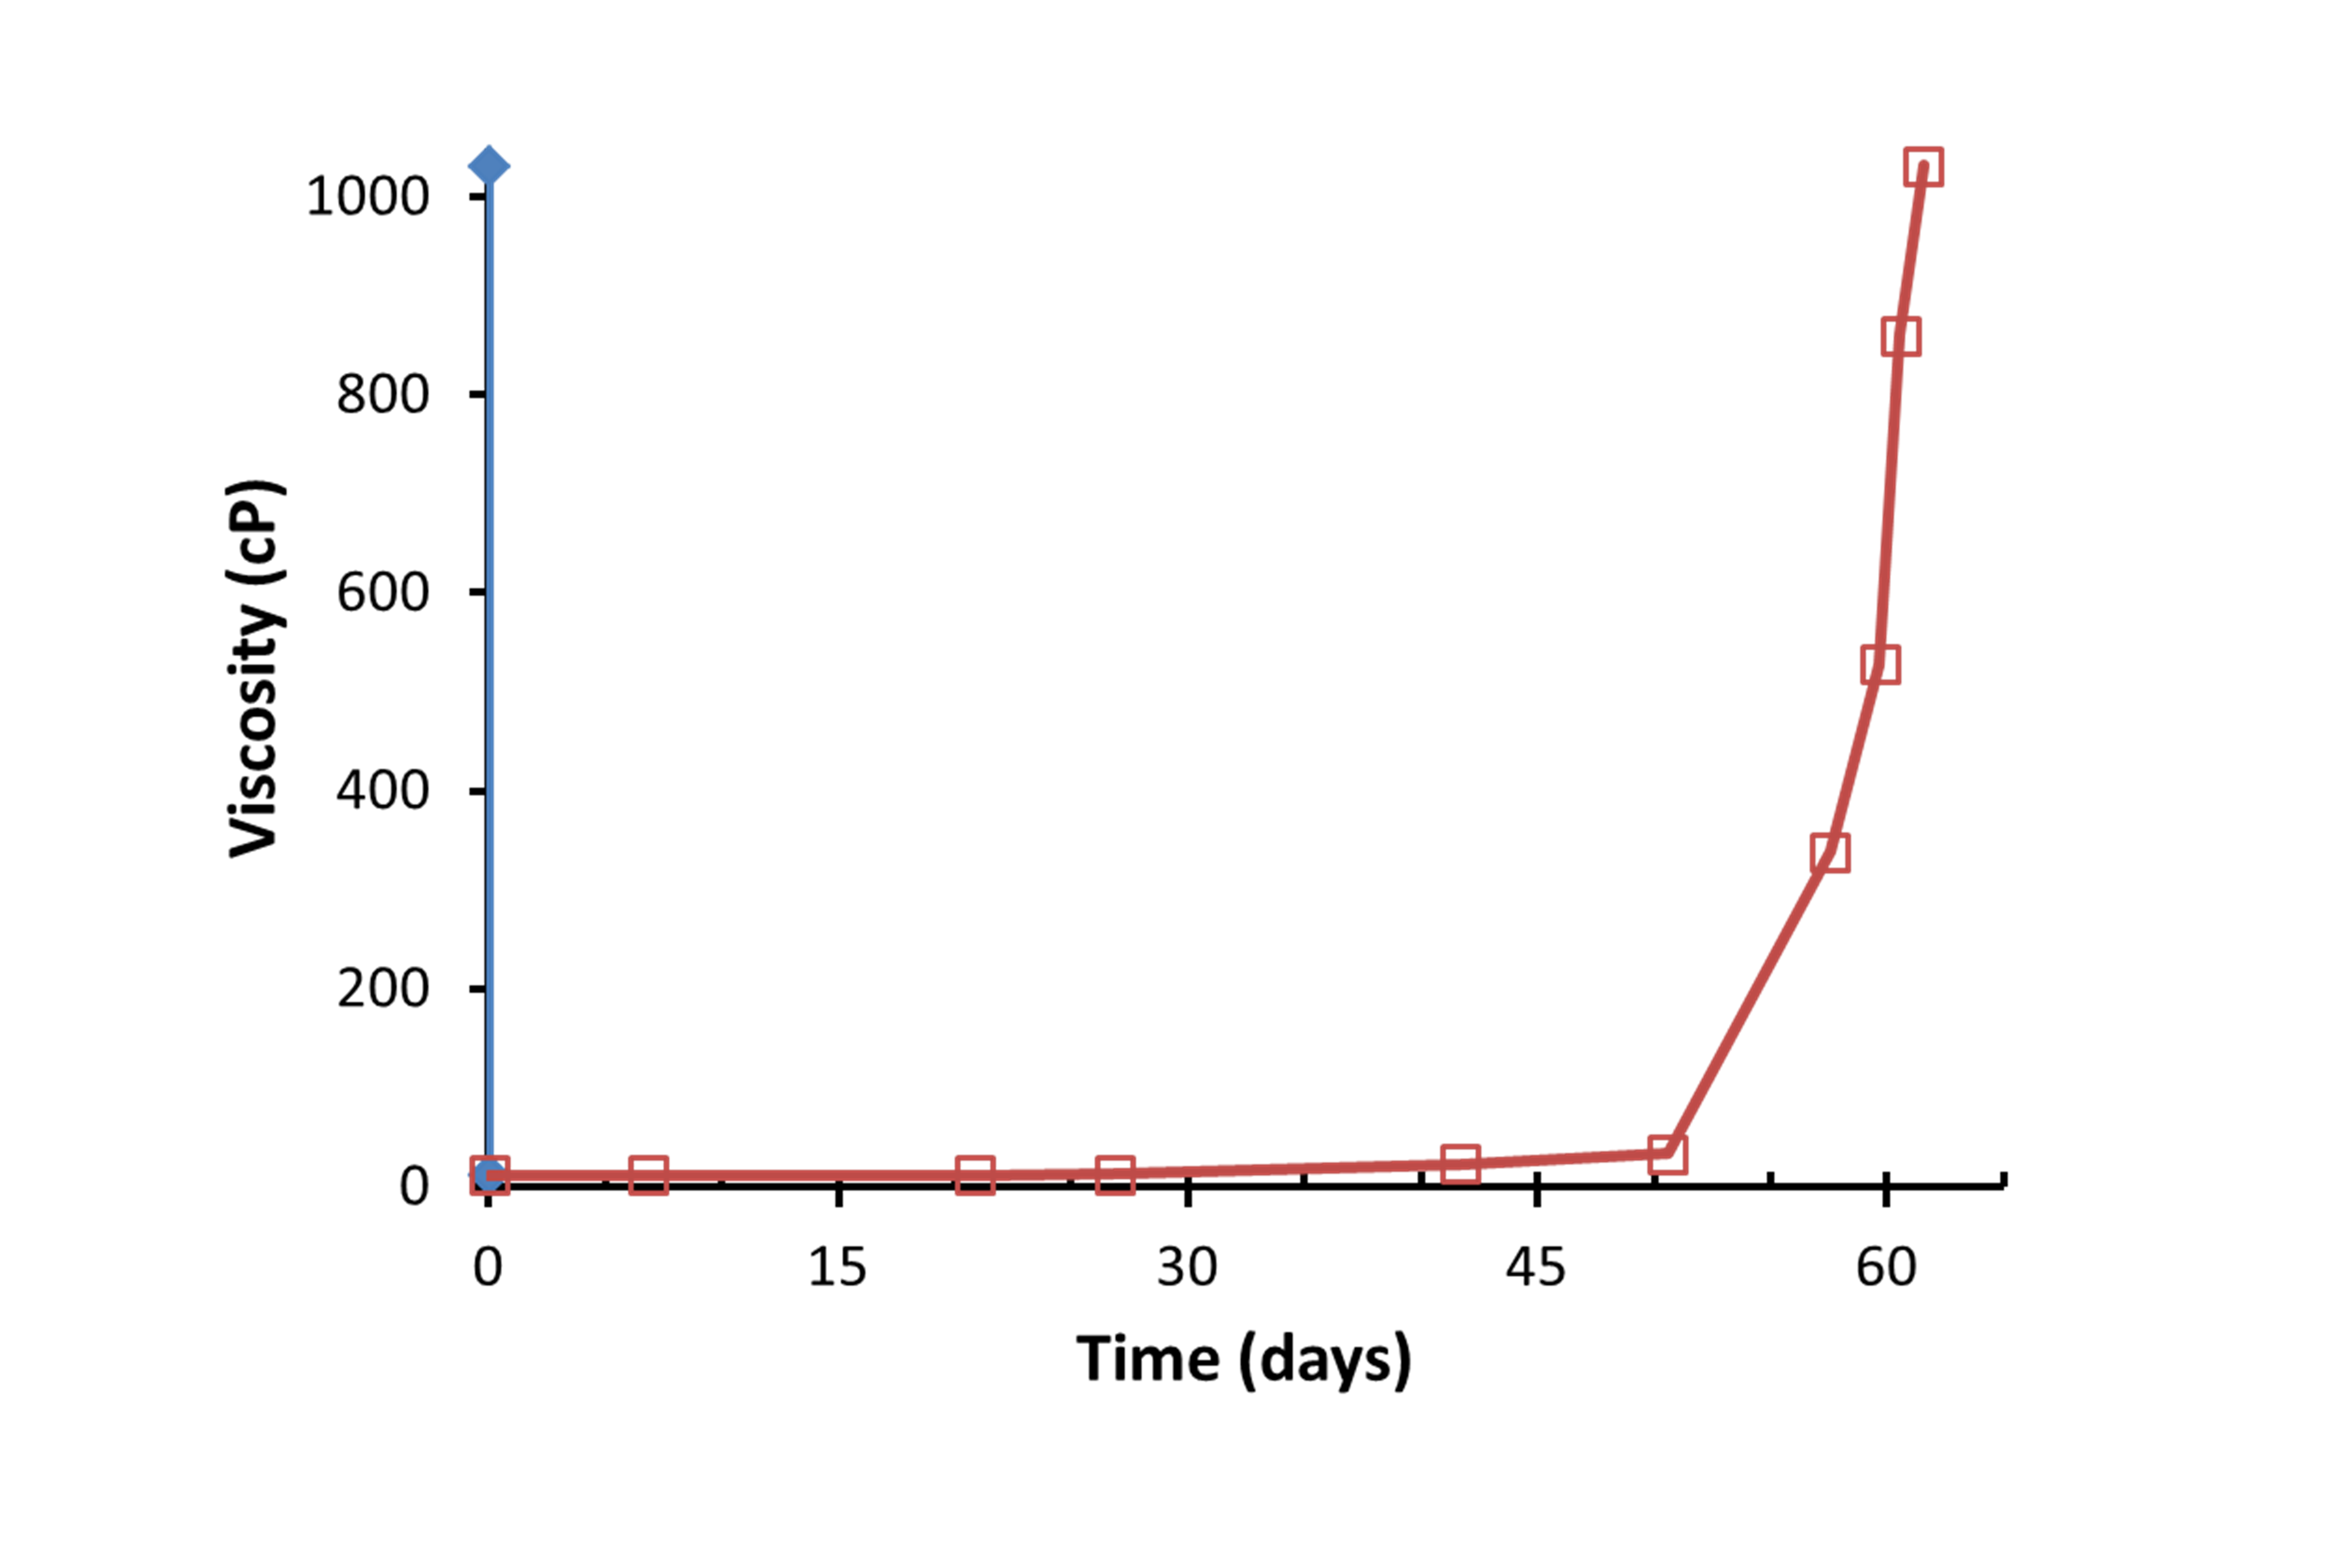
\includegraphics[width=.75\textwidth]{img/cht/jennTai.png}
    \caption{System with delayed gelation based on Texas A\&M technology \citep{Cordova2008}}
    \label{cht:jennTai}
\end{figure}

\newpage
The experiments on PEC nanogels consisted of three stages:
\begin{enumerate}
    \item Preparing the system in question (polymer and added components);
    \item Aging samples at elevated temperatures for various aging times;
    \item Measuring the viscosity of each sample at different shear rates.
\end{enumerate}

\subsection{Preparation}
\subsubsection{Polyelectrolyte complexes according to the Texas A\&M recipe}
A few tests were conducted with PEC systems made after the recipe by \cite{Johnson2010}, in order to reproduce similar results. In this recipe, in addition to the polymer and cross binder \ce{Cr^3+} the main constituents are dextran sulphate (DS) \index{dextran sulfate} and polyethyleneimine (PEI)\index{polyethyleneimine}. 1 wt.\% of both components in pure water were prepared for making PEC solutions by adding 15.39 g of DS solution to 34.28 g of PEI solution under vigorous stirring. The DS solution was added quickly as a "shot" by use of a syringe.
 
After approximately one minute of stirring, 1.13 g of a 10 wt.\% \ce{CrCl3.6H2O} was added. The final solution was made by first mixing 5.38 g of a 4 wt.\% Alcomer 24 UK solution (in SSW\index{synthetic sea water}) with 25.35 g of SSW. Next, this polymer solution was mixed with 12.32 g of the PEC solution. The concentration of polymer and \ce{Cr^3+} in the final solution were 0.499 wt.\% and 129 ppm, respectively. The samples were aged at 50~\celsius. The sample series was named Series 10.

Two more series of polymer/PEC solutions were made using 0.498 wt.\% and 0.490 wt.\% of Alcomer 24 UK (Series 35) and Flopaam 5115 VHM (Series 36), respectively. The composition of the PEC was as described above. The concentrations of \ce{Cr^3+} in the two solutions were 119 ppm and 115 ppm. The solutions were aged at 80~\celsius. 

Yet another two systems were made in an equivalent manner using Alcomer 24 UK, but with reduced concentrations of \ce{Cr^3+} (60 ppm in Series 42 and 41 ppm in Series 47). Table \what shows a summary of prepared systems using the Texas A\&M recipe [MAKE TABLE!\what]

\subsubsection{Polyelectrolyte complexes based on amine POSS}\index{polyhedral oligomeric silsequioxanes}

In PECs based on amine POSS the polycation PEI was replaced by the nanoparticle which also contains amine groups. As suggested by researchers at Texas A\&M the DS was replaced by the polyanion polyvinyl sulfonate (PVS)\index{polyvinyl sulfonate}. Series 17 through 20 were made using this method (table \what).

The cores of the amine POSS are silicon oxide. 

\subsection{Aging}
Each prepared system was distributed into six vials (a through f) that were sealed with rubber stoppers and crimp seals, as shown in Figure \ref{fig:vials}. Then the vials were placed on a KS 500 shaker (Janke \& Kunkel, IKA WERK, Figure \ref{fig:shaker}) with 300 shakes/min. While being shaken, the vials were purged with argon for 60 minutes \why. Argon was delivered through a syringe needle penetrating the rubber gasket. It then exited the vial through another needle (see Figure \ref{fig:argonPurge}).
\begin{figure}[p]
    \centering
    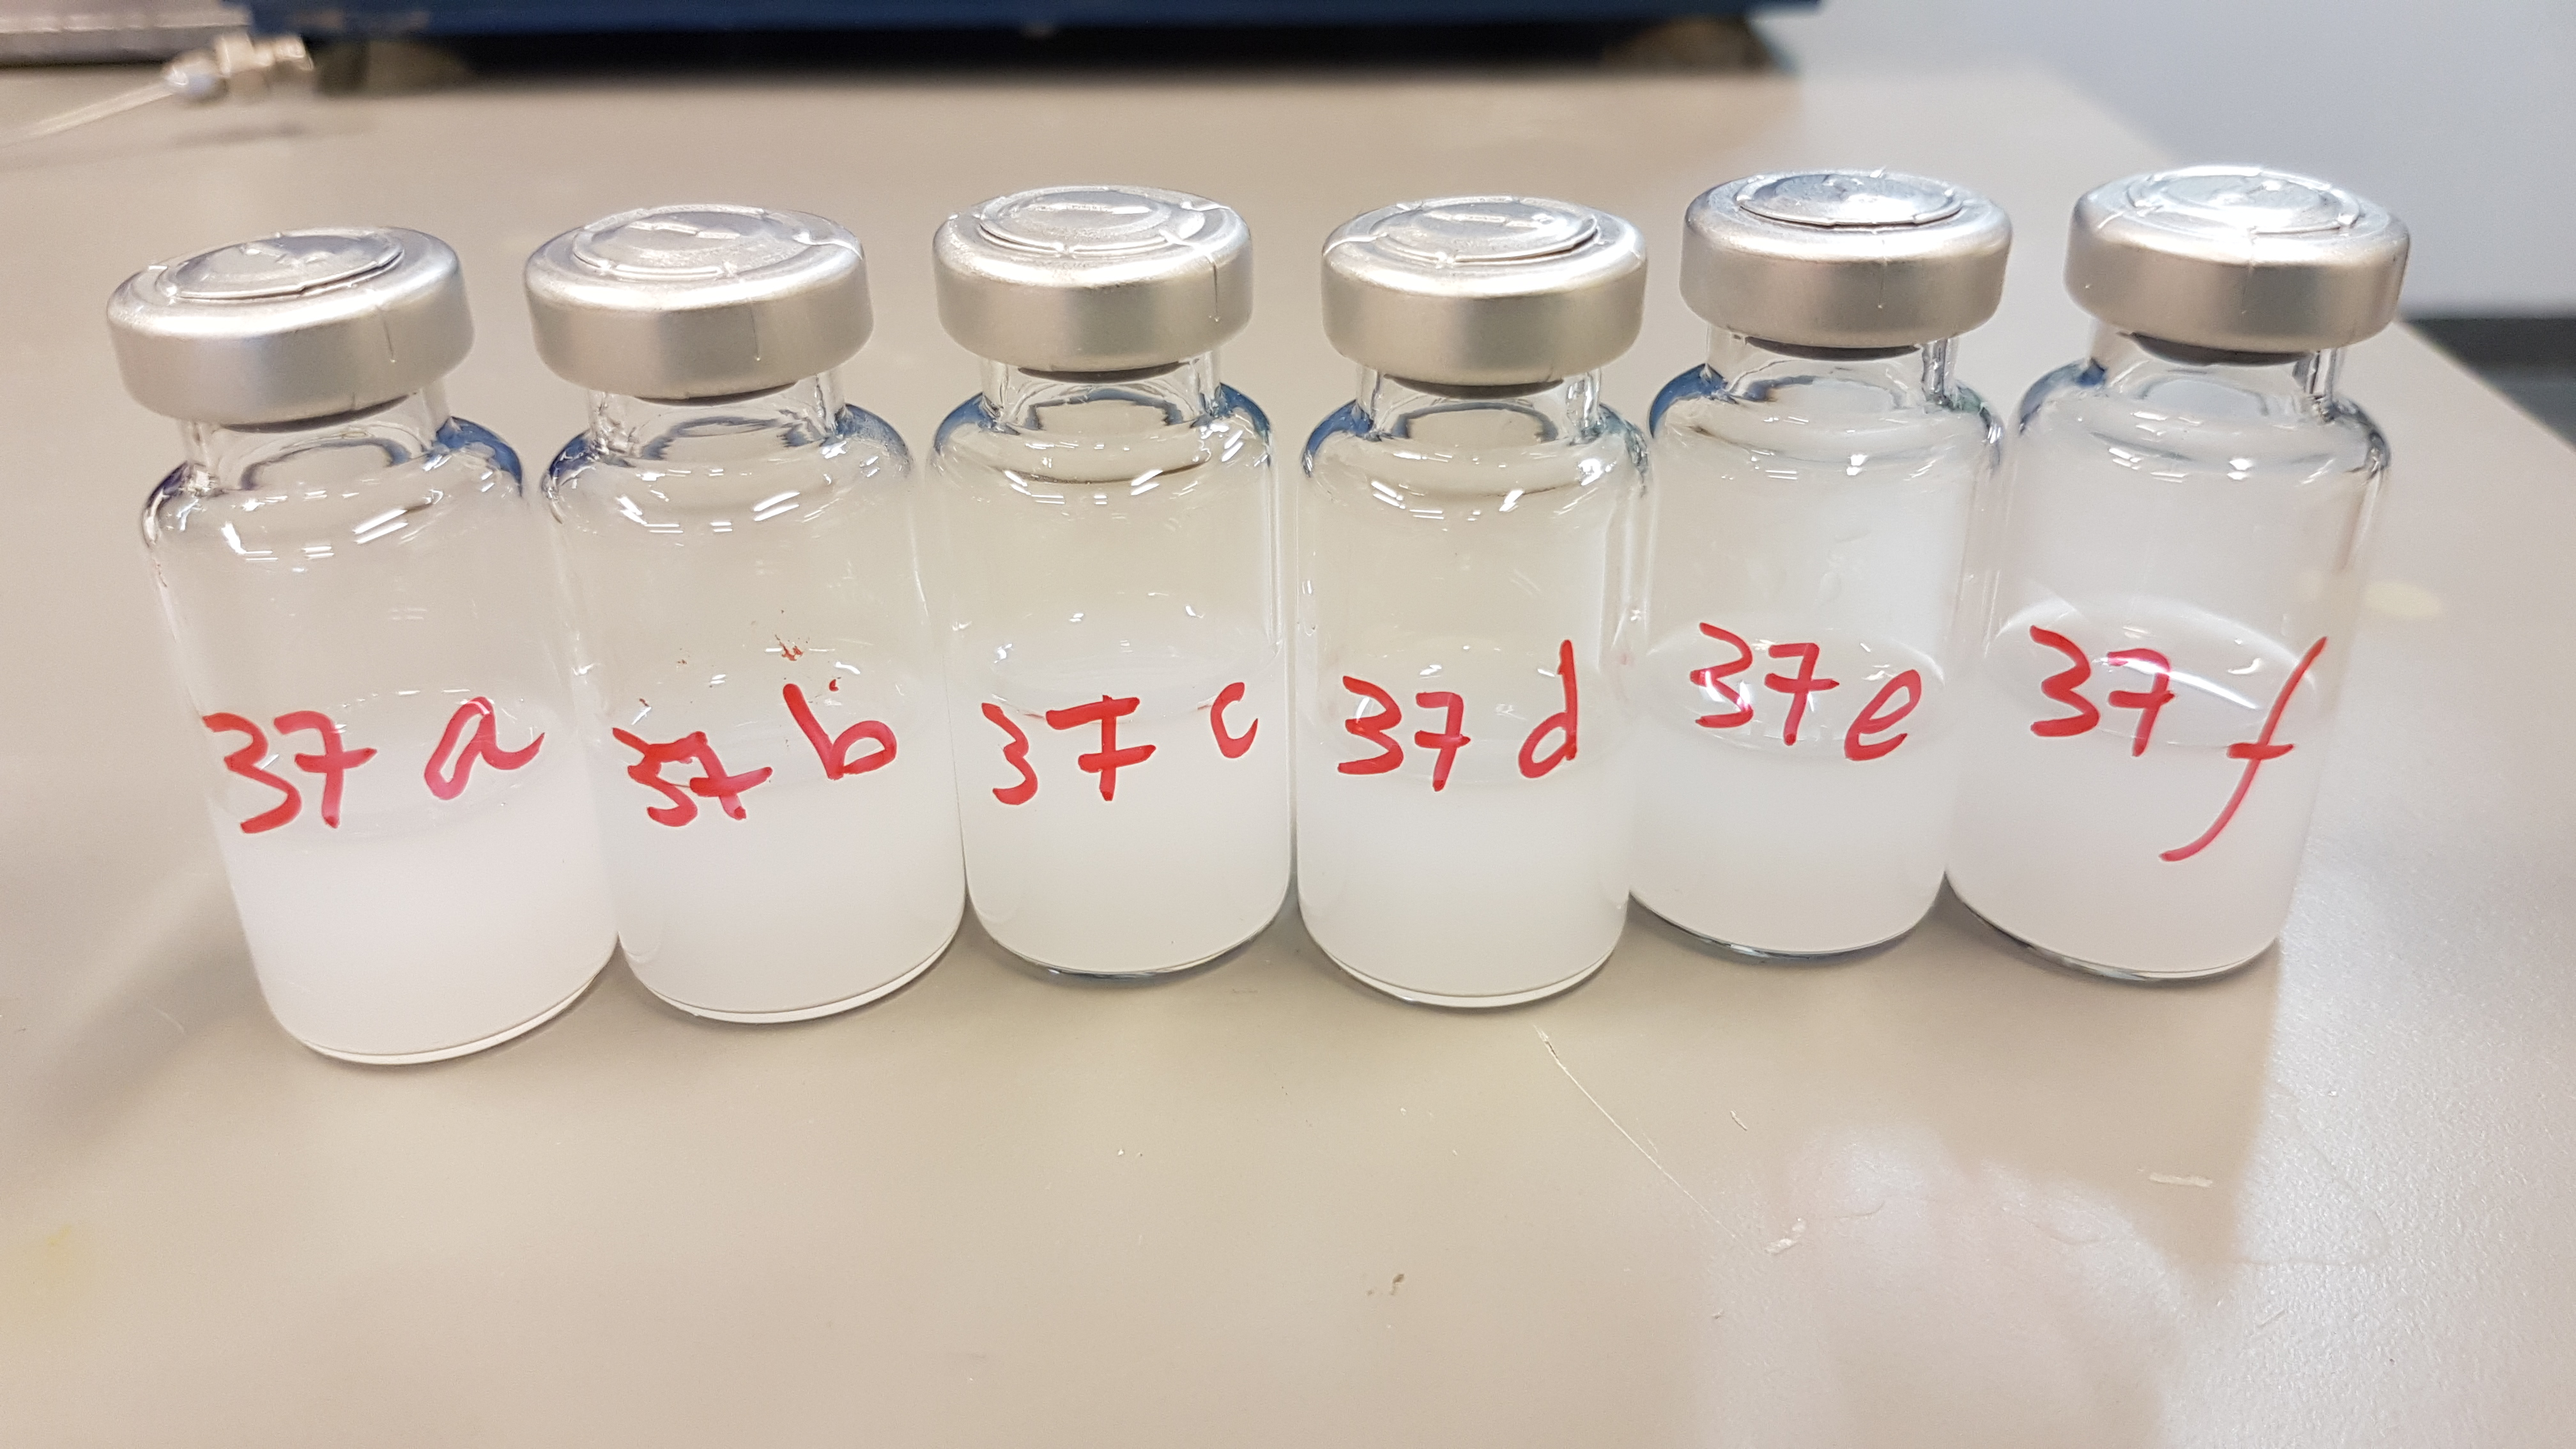
\includegraphics[width=.7\textwidth]{img/fig/vials.jpg}
    \caption{System \#37 distributed into vials ``a" through ``f" with rubber stoppers and crimp seals}
    \label{fig:vials}
\end{figure}
\begin{figure}[p]
    \centering
    \begin{subfigure}{0.45\textwidth}
        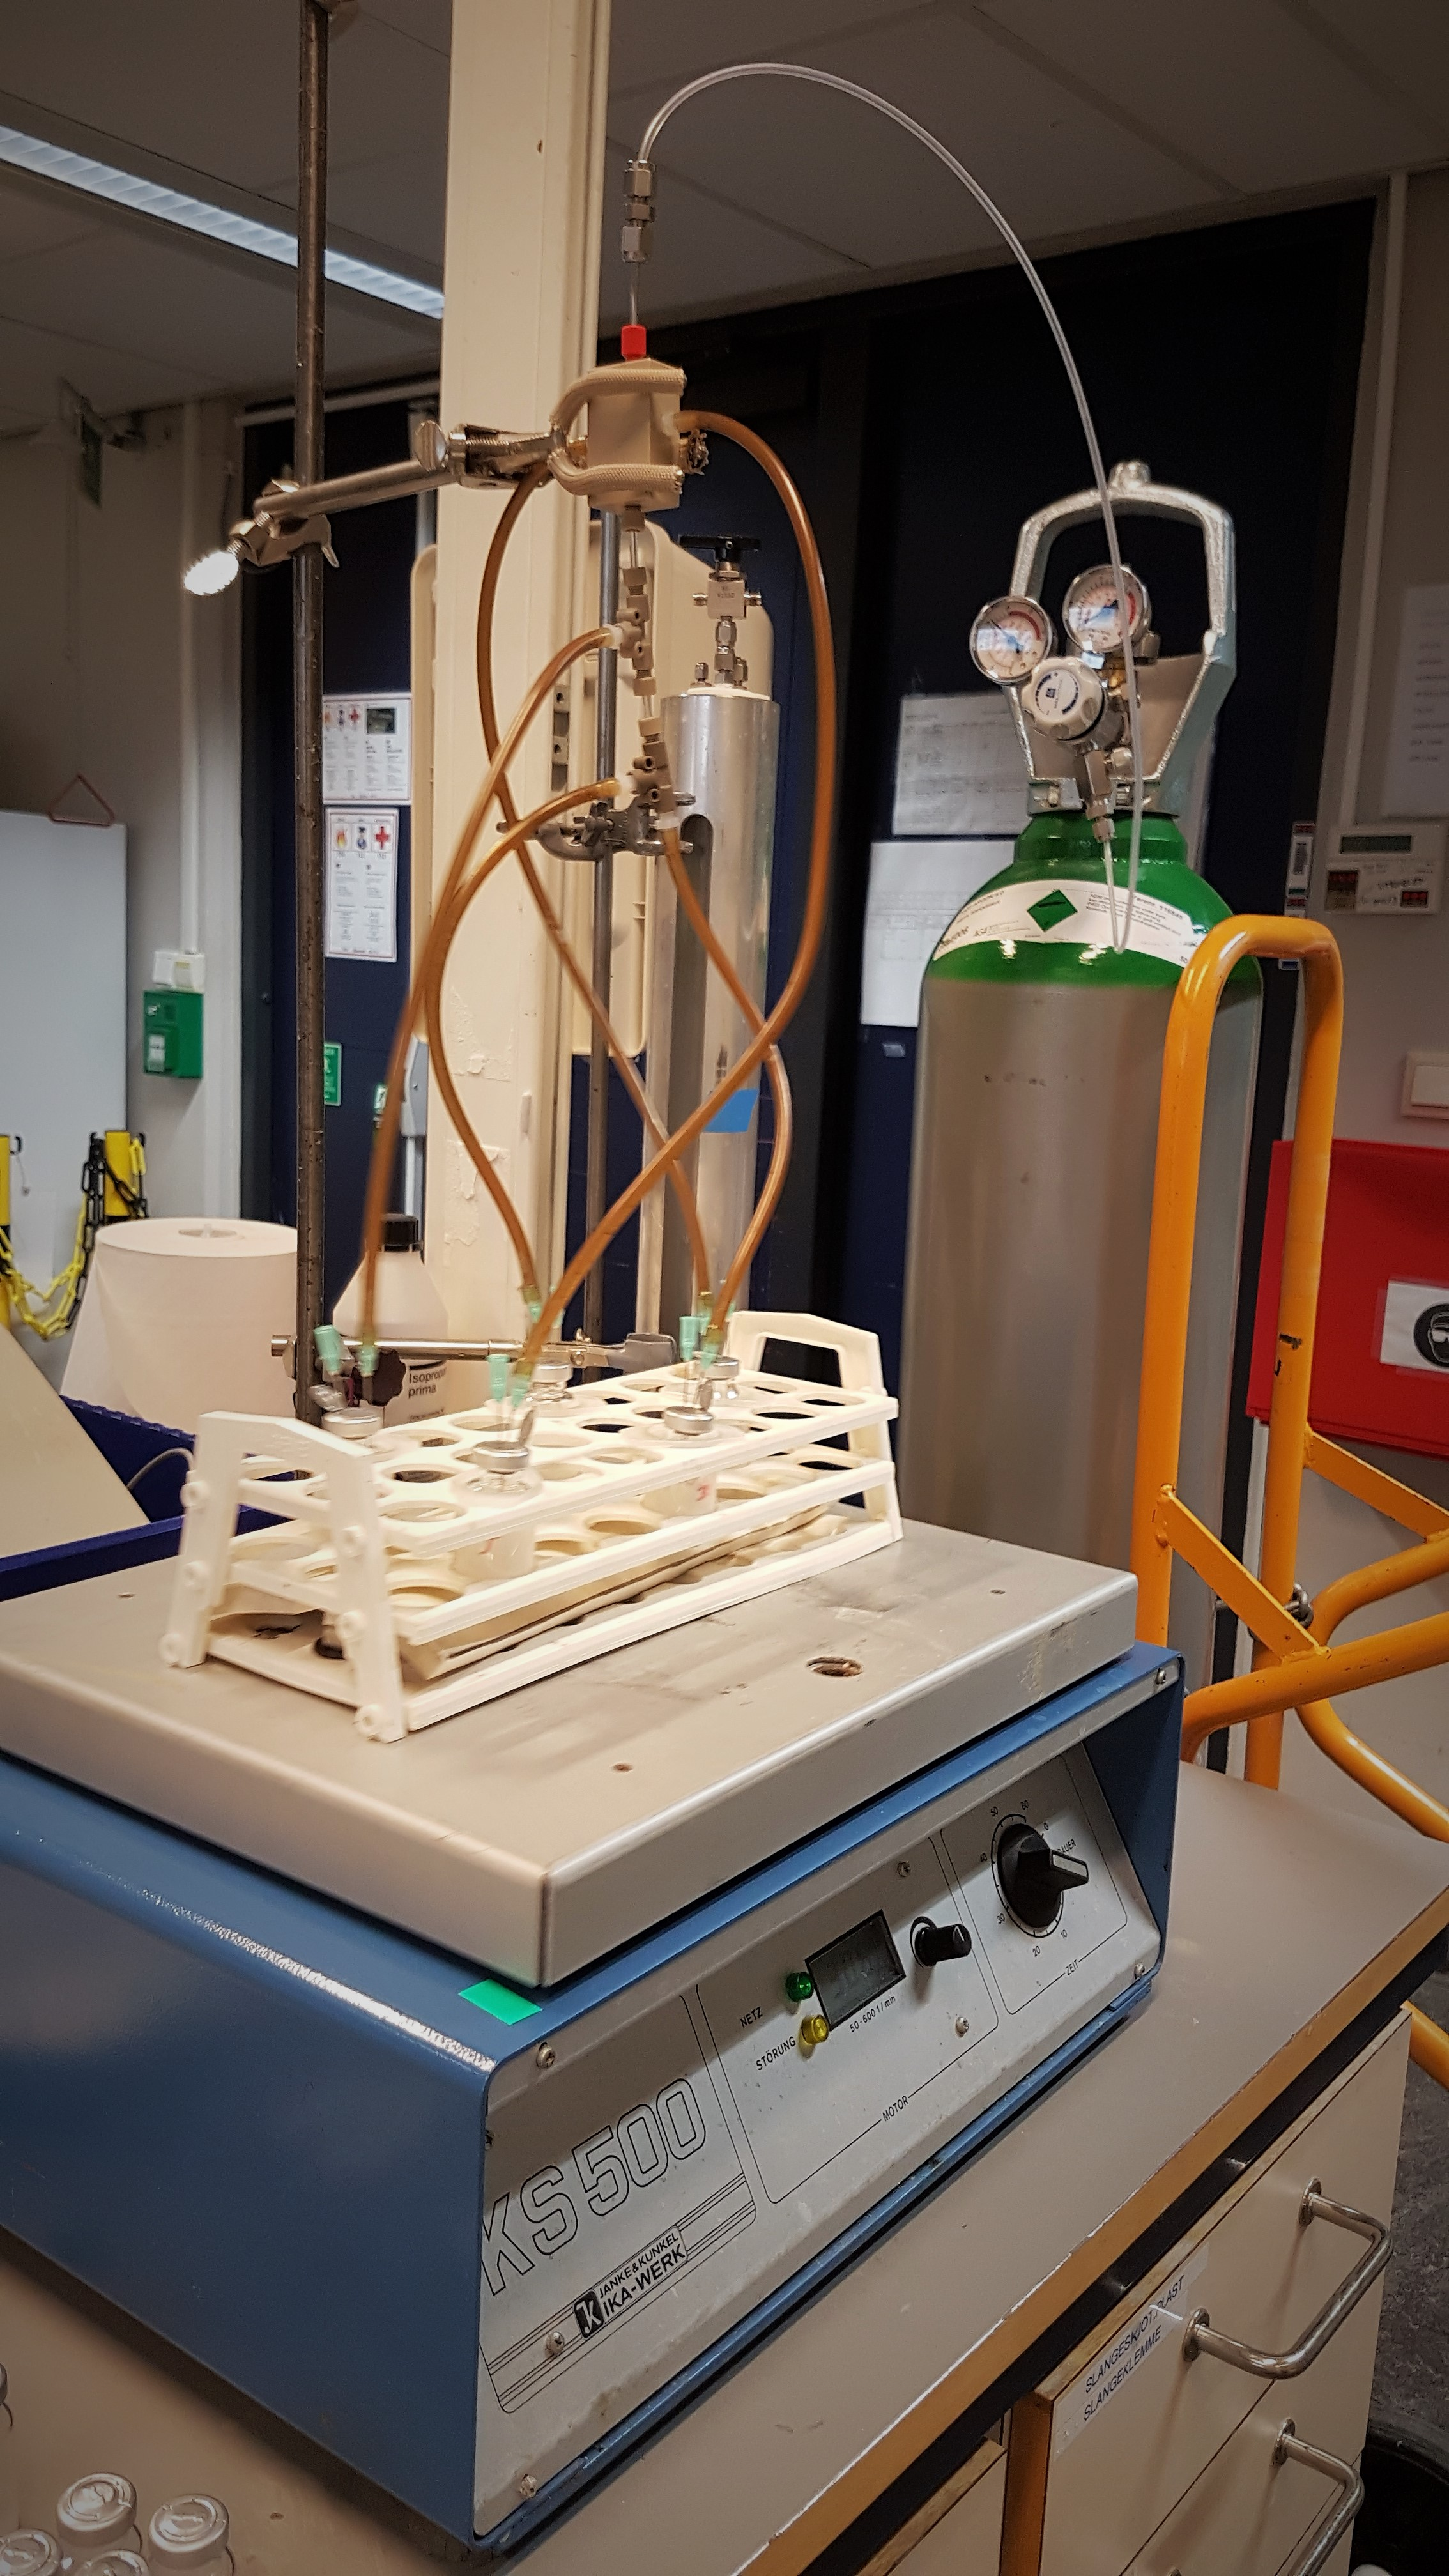
\includegraphics[width=\linewidth]{img/fig/shaker.jpg}
        \caption{} \label{fig:shaker}
    \end{subfigure}
    \hspace*{.05\textwidth} % separation
    \begin{subfigure}{0.45\textwidth}
        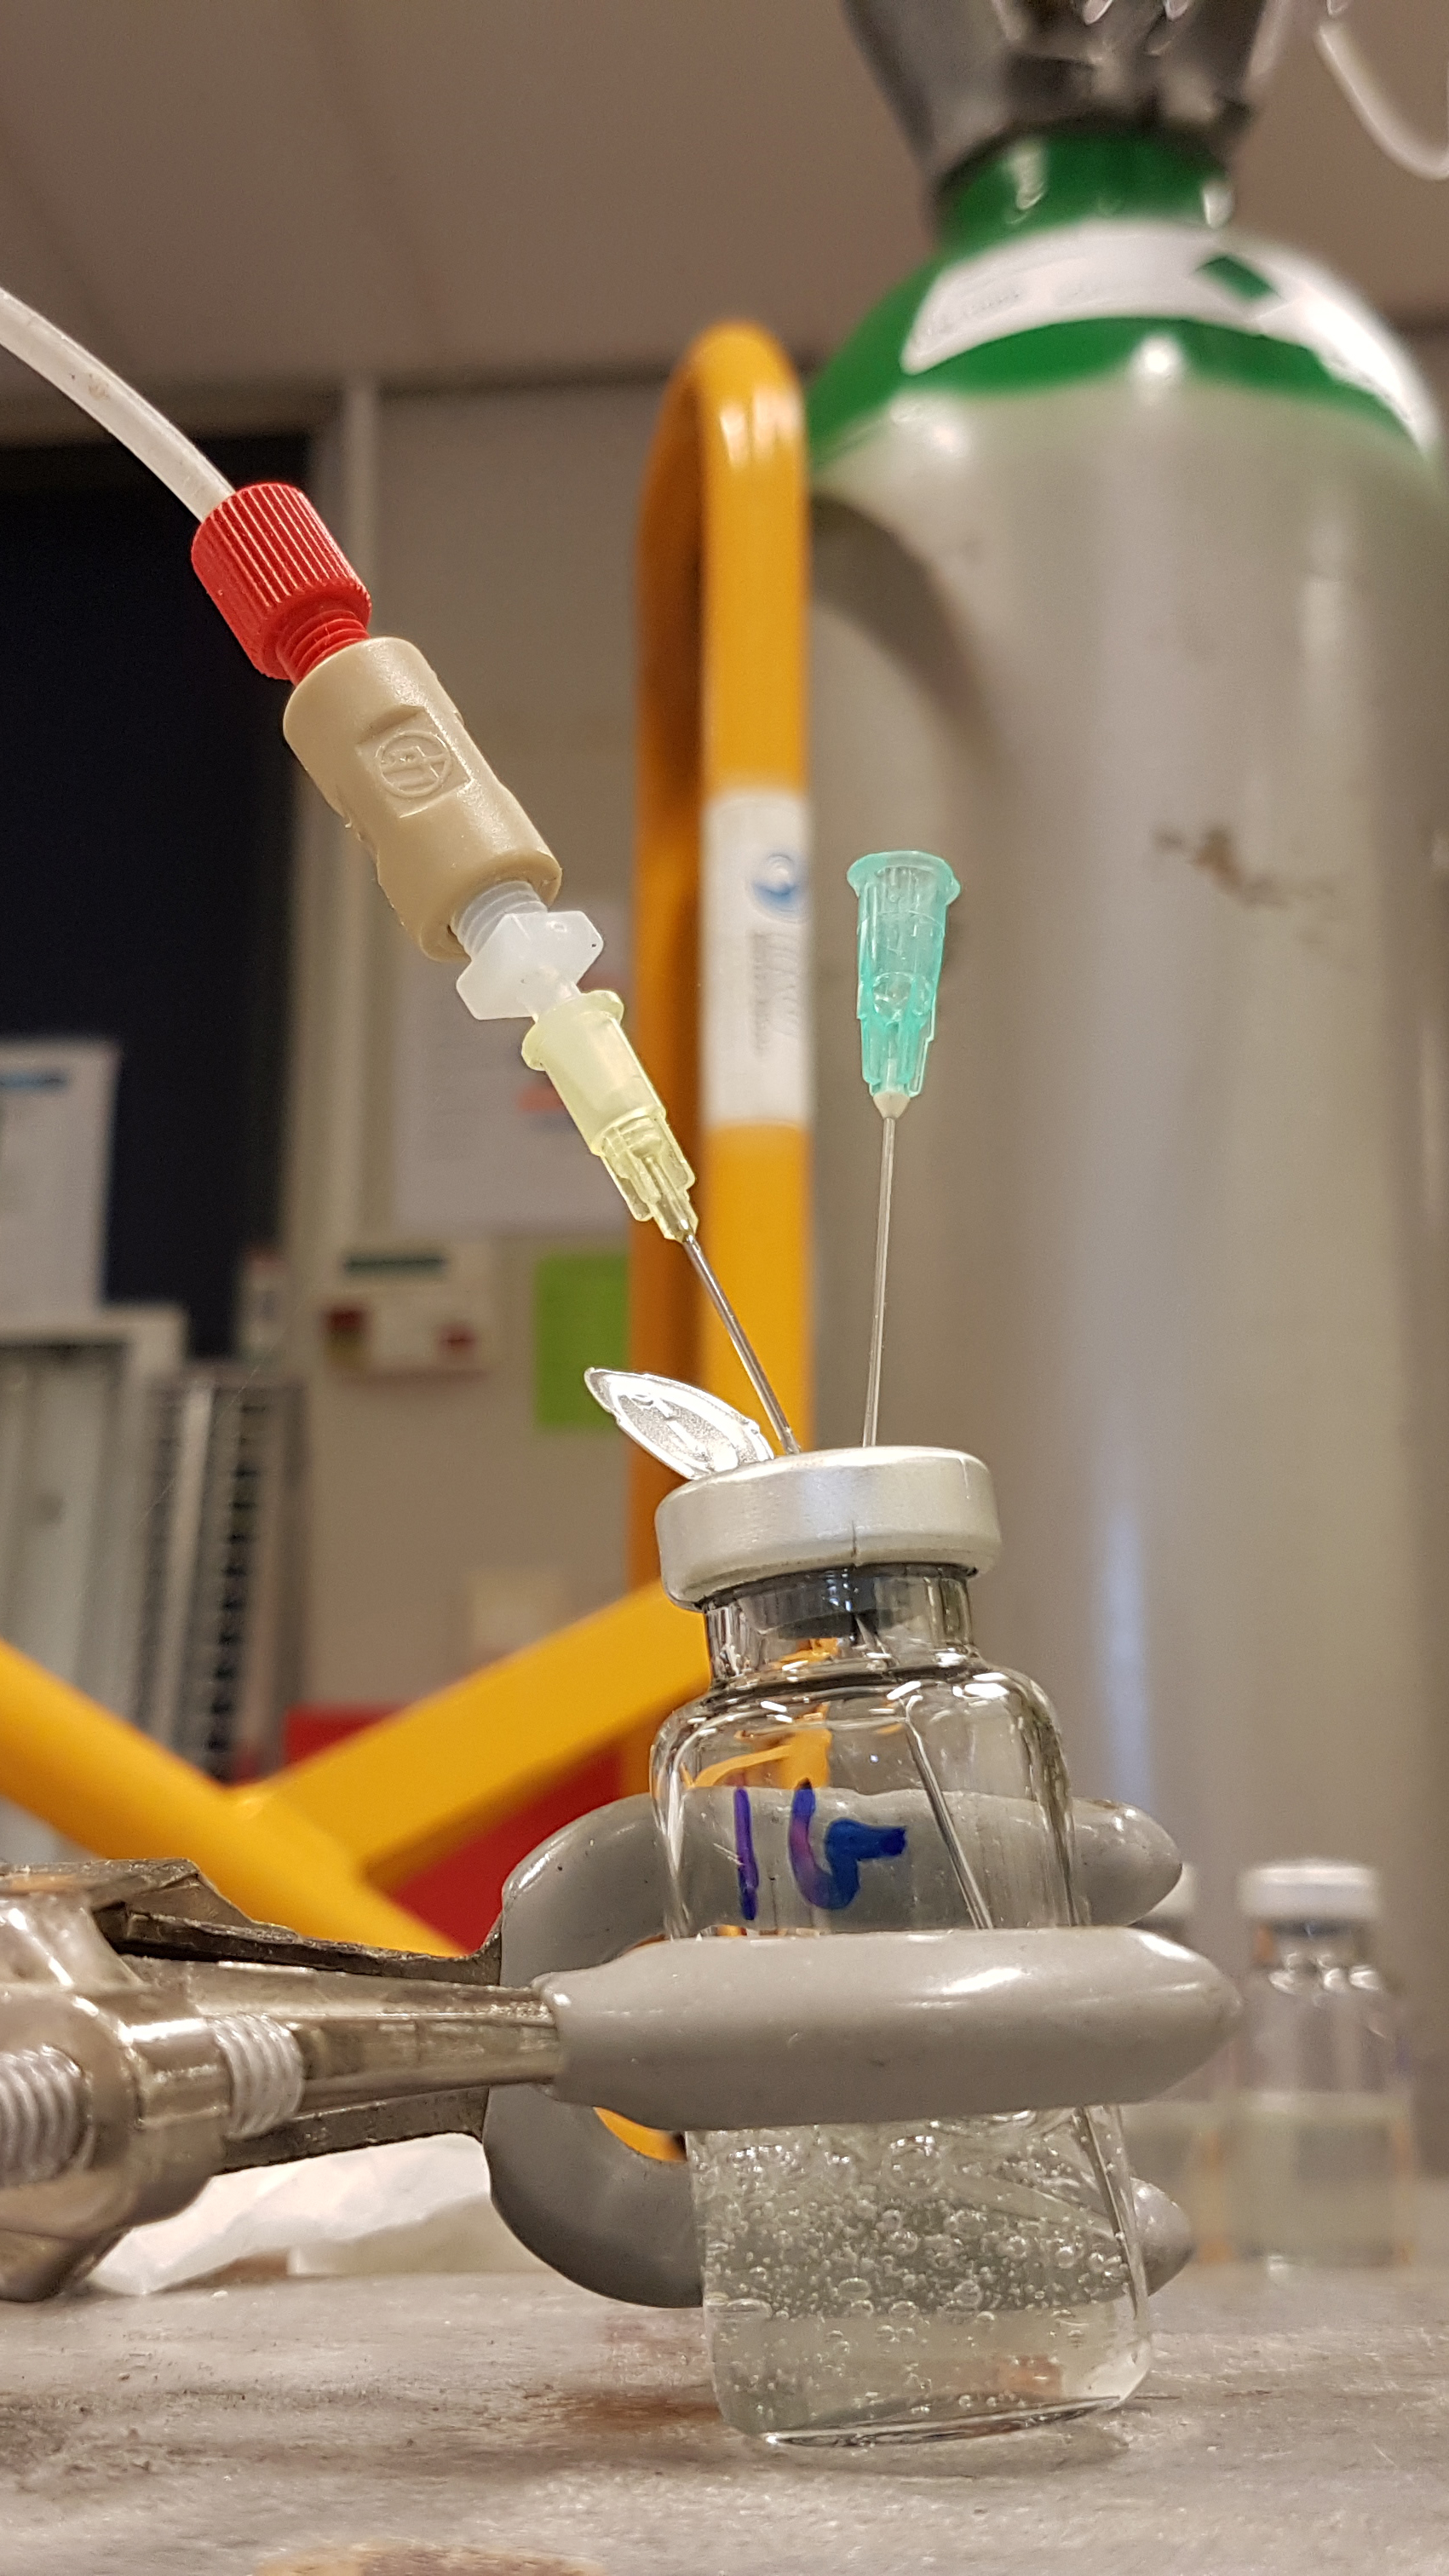
\includegraphics[width=\linewidth]{img/fig/argonPurge.jpg}
        \caption{} \label{fig:argonPurge}
    \end{subfigure}
    \caption{Purging samples with argon over a KS 500 shaker. (a) Shaker and argon cylinder (b) Argon purging syringe system with input and output needles}
    \label{fig:shaking}
\end{figure}

After the purging, samples were placed in an oven and were heated to 50~\celsius~(the first 16 series) and later at 80~\celsius~ \why. The ``a" sample from each series was not heated, and its viscosity was measured a short time after preparation. Samples ``b" through ``f" were kept in the oven, each for an exponentially increased aging time \why. 

\subsection{Viscosity measurement}
The viscosities of samples were measured using an Anton Paar MCR 302 rheometer (Figure \ref{fig:antonPaar}) under ambient conditions \why. After a sample was taken out of the oven, it was quickly transferred to the rheometer station, after which its viscosity was measured using a plate and cone geometry \why.

\begin{figure}[h]
    \centering
    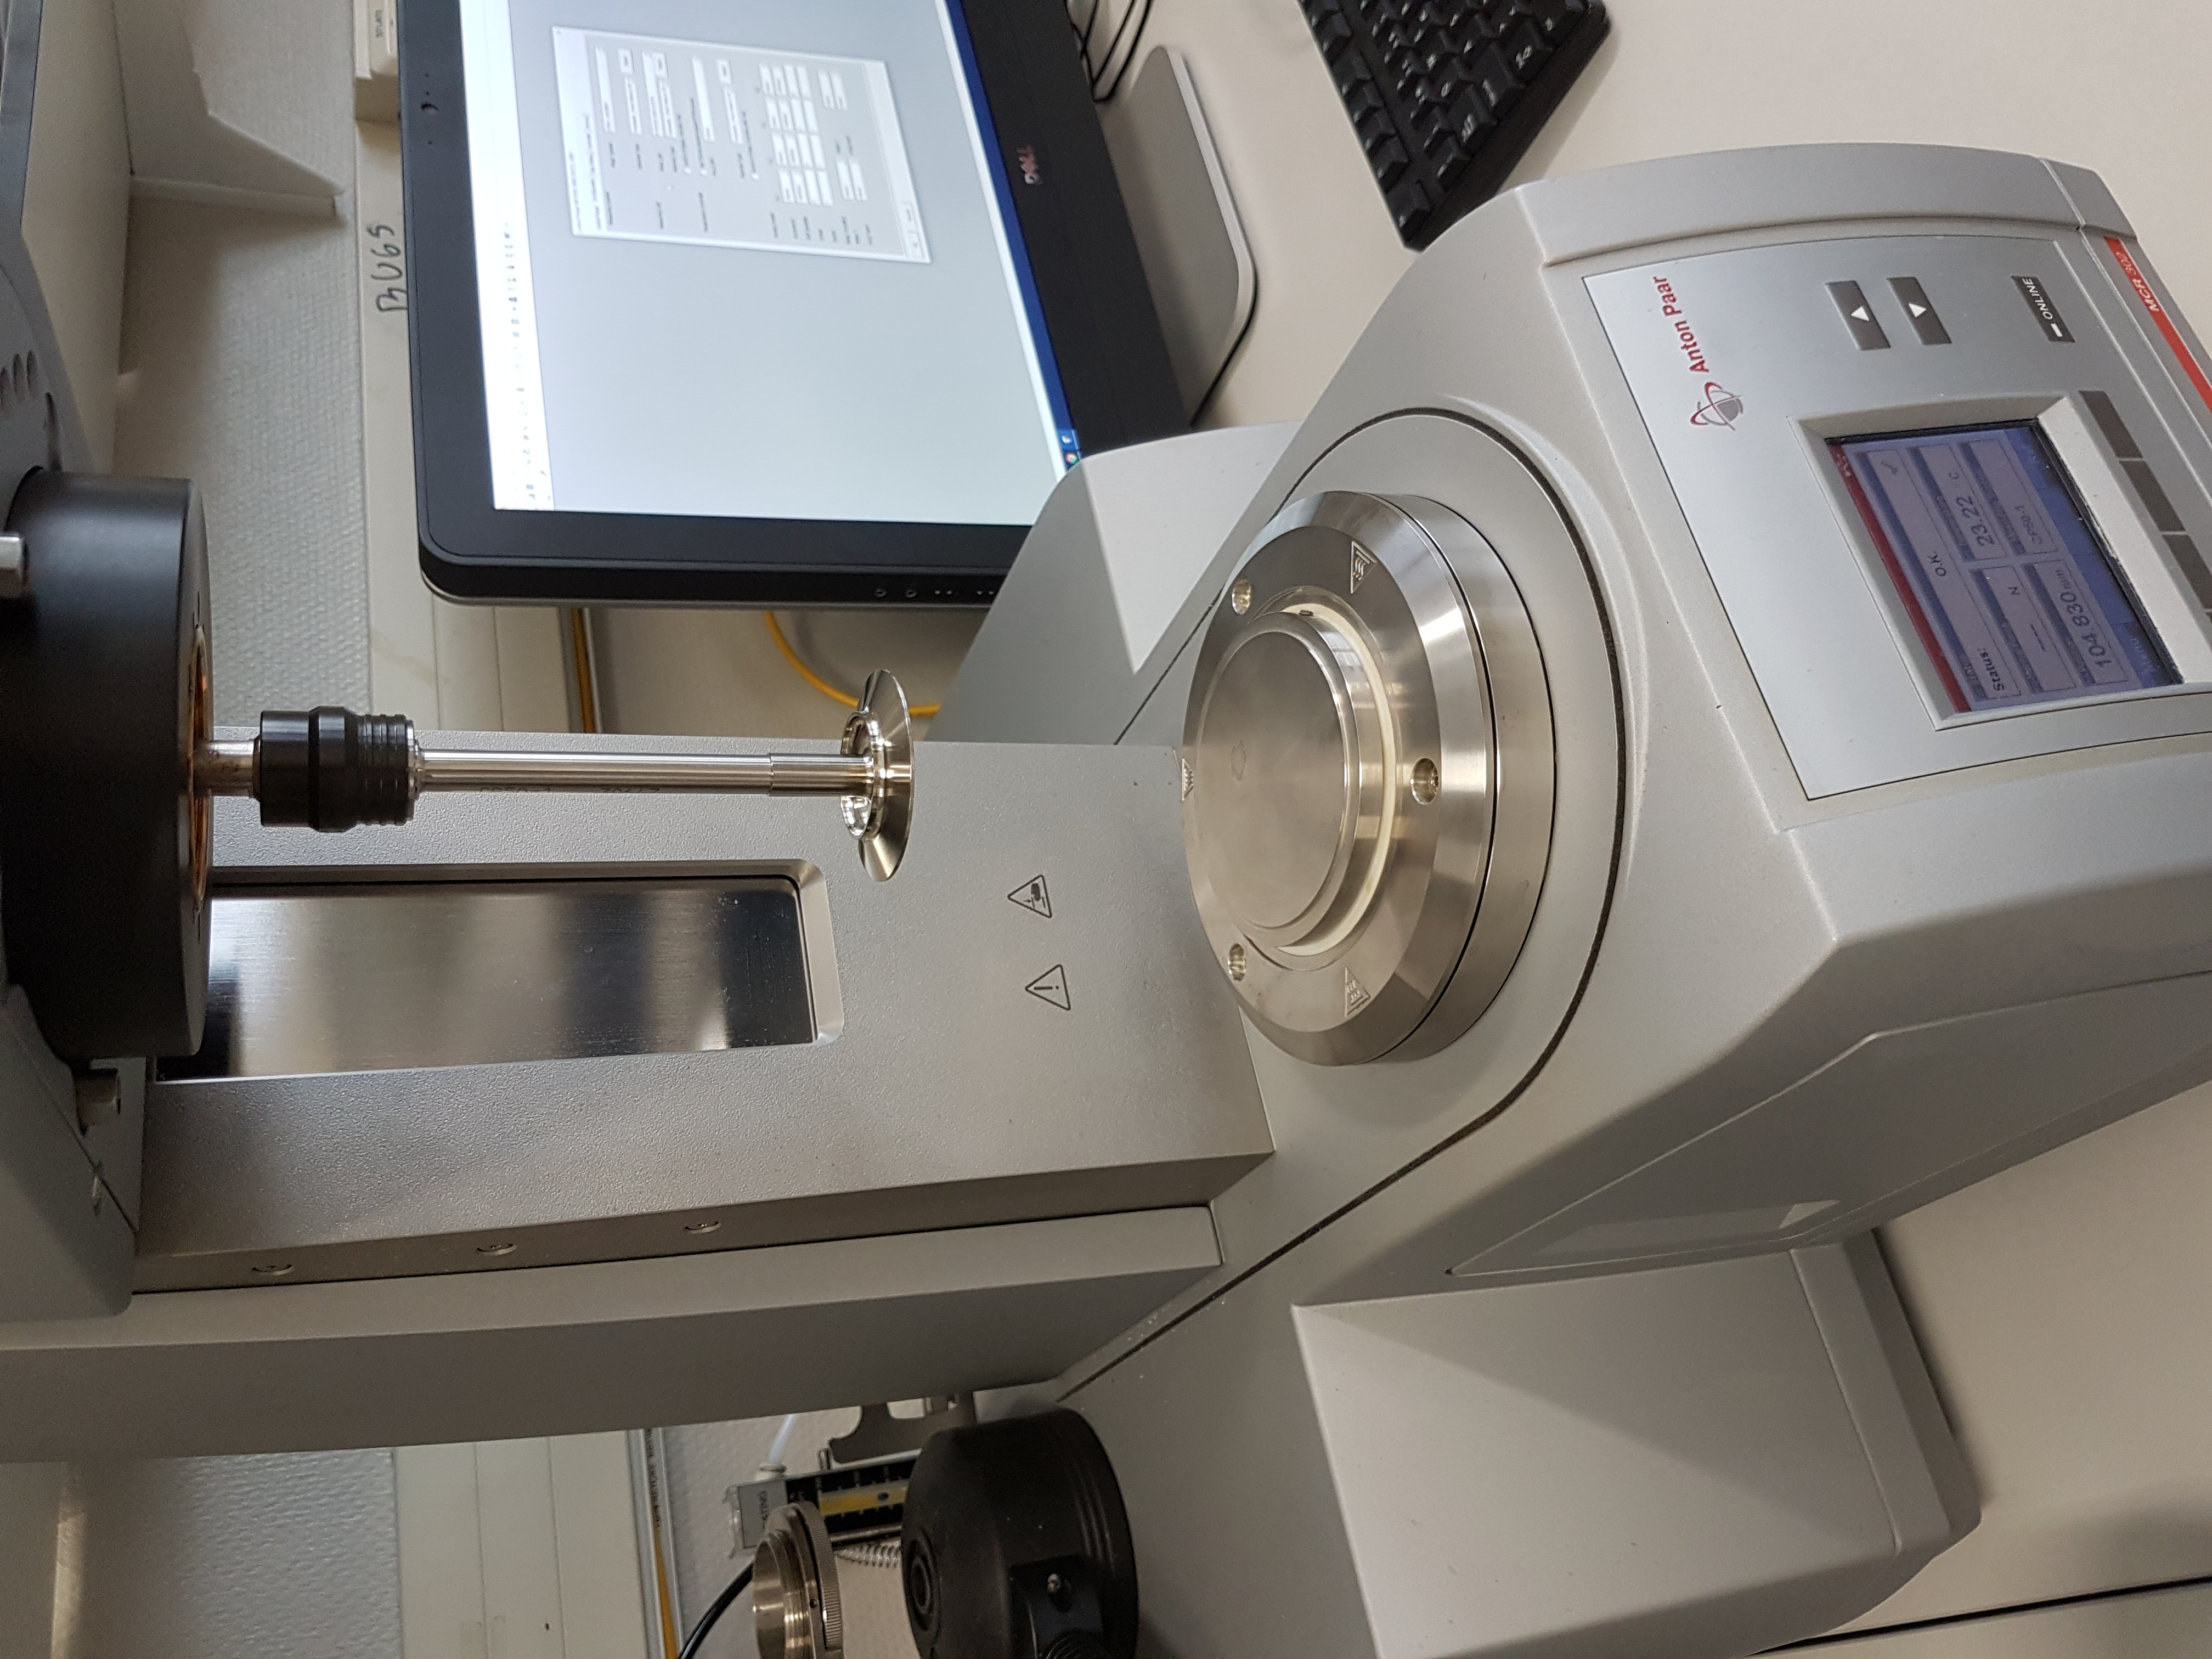
\includegraphics[width=.5\textwidth, angle=270]{img/fig/antonpaar.jpg}
    \caption{Anton Paar MCR 302 rheometer}
    \label{fig:antonPaar}
\end{figure}

The measurement procedure using the rheometer is as follows. First, a sample of suitable size was put on the plate. After that, the cone was lowered down onto the sample, until the sample spread into a thin film which completely filled the space between the cone and the plate. The measurement was then started according a preset schedule for shear rates. 

After initiating measurements, the instrument imposed a torque on the plate by rotating the cone at an initial slow speed, which was necessary to apply the first shear rate. The rotation lasted for the measurement time which was set to 2 seconds \why. After the measurement time had elapsed, the torque was increased to reach the next shear rate. The shear rates ranged from \what to \what and \what measurements with exponential increase in shear rates were made within this range. From the resulting torques and shear rates a relationship between viscosity and shear rate (shear curve) was then calculated by the software.

Admittedly, measuring shear curves is not the ultimate way of characterizing gel systems after gelation has started. Weak gels may be broken down during the shearing. For stronger gels, the velocity gradient between the measuring geometry will not be as homogeneous as in a weaker, more fluid gel, since it will only be over a small gap between the measurement bodies (cone and/or plate) and the gel. For such systems, other types of measurements can be used to get more accurate results, e.g. oscillatory measurements. Thus, the measurements presented in this chapter are at best semi-quantitative after gelation had started. However, valuable results were collected from said measurements.

Some operational issues arose in the process. For some systems, after gels were formed, it was difficult or impossible to remove the gel from the vial. After extracting such samples from vials, it was possible to obtain a shear curve for some systems. Other systems would not stay in place and slipped away when the cone was lowered onto the sample on the plate.
